\section{Test}

In the project, our team conducted a black box test on the file synchronization tool. At the beginning, our team tested the transmission of different kinds of file names and file formats. As shown below (Table Black box test result at the beginning). As you can see from the table, we have file names under different language specifications, file names with special symbols, and different types of file formats, such as zip, png, and docx etc. used to do the upload, download, delete and rename function tests. For the uploading, downloading and deleting of files, all the objects we tested can be implemented successfully. However, for the rename function, file names with Chinese names and special symbols cannot be renamed. \\\\
At the end of the project, our system implemented automation synchronize function, and these files with Chinese names and special symbols finally achieved in rename function. We analyzed the reason why we couldn't achieve it before because the name of the renamed file needs to be written in the code when we originally developed the product function, and the name with Chinese characters may be inconsistent with the language environment in which the code is written. So, the function cannot be achieved.\\\\
Furthermore, we also learned and configuration test environment of Mocha, Chai and Sinon for the desktop application. We try to implement the jsunit test. But for some reasons, it is not complete.\\\\
Test case is show below:\\
\begin{minipage}
\centering
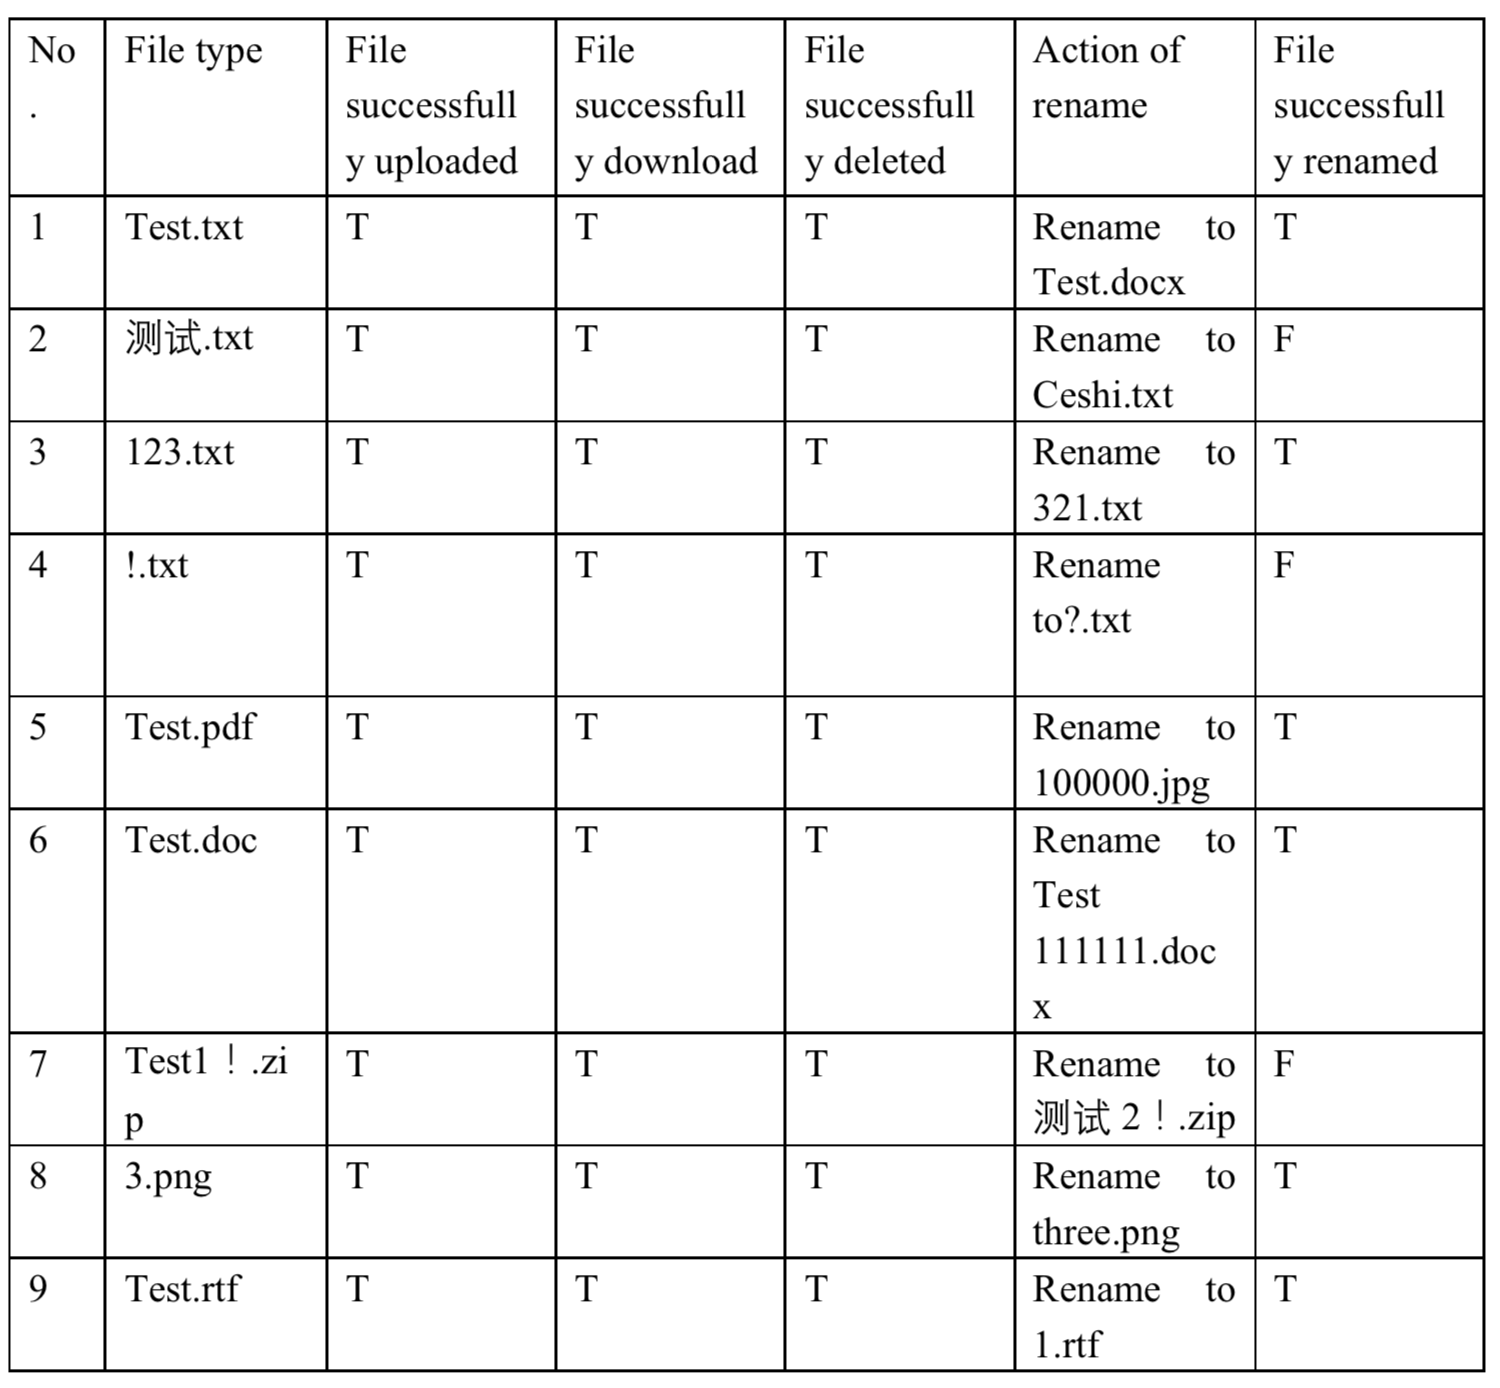
\includegraphics[scale=0.5]{test_case.png}

\label{fig:test_case}
\end{minipage}
